\documentclass[10pt,landscape]{article}
\usepackage{multicol}
\usepackage{calc}
\usepackage{ifthen}
\usepackage[landscape]{geometry}
\usepackage{verbatim}
\usepackage{graphicx}

\usepackage{color}
\usepackage[usenames,dvipsnames,svgnames,table]{xcolor}
\usepackage{menukeys}

\usepackage{hyperref}
\hypersetup{colorlinks=true}

% Narrow margins
\ifthenelse{\lengthtest { \paperwidth = 11in}}
	{ \geometry{top=.5in,left=.5in,right=.5in,bottom=.5in} }
	{\ifthenelse{ \lengthtest{ \paperwidth = 297mm}}
		{\geometry{top=1cm,left=1cm,right=1cm,bottom=1cm} }
		{\geometry{top=1cm,left=1cm,right=1cm,bottom=1cm} }
	}

% Turn off header and footer
\pagestyle{empty}
 
% Redefine section commands to use less space
\makeatletter
\renewcommand{\section}{\@startsection{section}{1}{0mm}%
                                {-1ex plus -.5ex minus -.2ex}%
                                {0.5ex plus .2ex}%x
                                {\normalfont\large\bfseries\center\color{RoyalBlue}}}
\renewcommand{\subsection}{\@startsection{subsection}{2}{0mm}%
                                {-1explus -.5ex minus -.2ex}%
                                {0.5ex plus .2ex}%
                                {\normalfont\normalsize\bfseries\center\color{Cerulean}}}
\renewcommand{\subsubsection}{\@startsection{subsubsection}{3}{0mm}%
                                {-1ex plus -.5ex minus -.2ex}%
                                {1ex plus .2ex}%
                                {\normalfont\small\bfseries\center\color{ForestGreen}}}
\makeatother

% Highlighted text
\newcommand{\hilight}[1]{\colorbox{yellow}{#1}}

% Don't print section numbers
\setcounter{secnumdepth}{0}


\setlength{\parindent}{0pt}
\setlength{\parskip}{0pt plus 0.5ex}


% -----------------------------------------------------------------------

\begin{document}

\raggedright
\footnotesize
\begin{multicols}{3}

% multicol parameters
% These lengths are set only within the two main columns
%\setlength{\columnseprule}{0.25pt}
\setlength{\premulticols}{1pt}
\setlength{\postmulticols}{1pt}
\setlength{\multicolsep}{1pt}
\setlength{\columnsep}{2pt}

\begin{center}
     
\includegraphics[width=7em]{vim_logo.eps}
     \Large{\textbf{\color{WildStrawberry}{Cheat Sheet}}} \\
\end{center}

\section{Bare minimum}
\subsection{Start editing...}
\begin{tabular}{@{}ll@{}}
\verb!i!       & At the cursor \\
\verb!I!       & At the first non-whitespace of the line \\
\verb!a!       & After the cursor \\
\verb!A!       & After the last character of this line \\
\verb!o!       & New line after this one\\
\verb!O!       & New line before this one\\
\end{tabular}

\subsection{Navigation}
\subsubsection{Line scope}
\begin{tabular}{@{}ll@{}}
\verb!^!          	& Goto first non-whitespace char in line\\
\verb!$!          	& Last character in line\\
\verb!e (E)!      	& End of (whitespace-delimited) \hilight{word}, next word\\
\verb!b (B)!      	& Beginning of (whitespace-delimited) \hilight{word}, last word\\
\end{tabular}

\subsubsection{Document scope}
\begin{tabular}{@{}ll@{}}
\verb!:n!         	& Goto line number \verb!n!\\ 
\verb![m!,\verb!]m! & Previous, next \hilight{method} (in Java and like)\\ 
\ctrl+b,f			& Previous, next \hilight{page}\\
\end{tabular}


\subsection{Copy, Paste, Delete}
\begin{tabular}{@{}ll@{}}
\verb!dd!      			& Delete this \hilight{line} \\
\verb!d$!, \verb!D!     & Delete till EOL \\
\verb!d10d!    			& Delete \hilight{10 lines} \\
\verb!y3w!     			& Copy 3 \hilight{words} \\
\verb!pp!      			& \hilight{Paste} deleted or copied text \\
\end{tabular}

\subsection{Search and Replace}
\begin{tabular}{@{}ll@{}}
\verb!/Romeo!		         & Search for \verb!Romeo!\\
\verb!/\cromeo!		         & Search for \verb!Romeo!, \hilight{case insensitive} \\
\verb!:g/Romeo/#!			 & 
\includegraphics[width=1em]{../img/happy.png}Show matches with line numbers\\
\verb!n!   		             & Next match\\
\verb!N!		             & Previous match\\
\verb!:%s/old/new/!          & \hilight{Replace} \verb!old! with \verb!new! globally\\
\verb!:%s/old/new/c!         & Ask for every match\\
\verb!:%s/^\s*--//!          & Remove SQL comments (\verb!--!)\\
\end{tabular}

\subsection{Undo and Redo}
\begin{tabular}{@{}ll@{}}
\verb!u!          & Undo\\
\end{tabular}

\subsection{Save and Quit}
\begin{tabular}{@{}ll@{}}
\verb!:w! 	        & Save\\
\verb!:wq!          & Save and quit\\
\verb!:q!!          & Quit discarding changes\\
\end{tabular}

\section{Nice to have}

\subsection{Code}

\subsubsection{Syntax Highlighting}
\begin{tabular}{@{}ll@{}}
\verb!:syntax {on|off}!      & Toggle syntax highlighting \\
\verb!:set bg={dark|light}!  & Adjust highlighting brightness \\
\end{tabular}

\subsubsection{Line numbers}
\begin{tabular}{@{}ll@{}}
\verb!:set (no)nu!				& Set (no) line numbers \\
\end{tabular}

\subsubsection{Indentation}
\begin{tabular}{@{}ll@{}}
\verb!==!				& Indent this \hilight{line} \\
\verb!50==! 		 	& Indent 50 next lines in accordance with this line \\
\verb!gg=G! 		 	& Indent \hilight{entire document} (\verb!gg! for start, \verb!G! for end) \\
\end{tabular}

\begin{center}
\rule{0.3\linewidth}{0.25pt}
\end{center}


\includegraphics[width=6em]{../img/by_nc_sa.eps} This work is licensed under a \href{http://creativecommons.org/licenses/by-nc-sa/3.0/}{Creative Commons Attribution-NonCommercial-ShareAlike 3.0 Unported License}.

{\copyright\ 2012 \href{http://matan.name}{Adam Matan}.}

\begin{tiny}
Sources: 	\href{http://rayninfo.co.uk/vimtips.html}{Best of Vim Tips},
			\href{http://people.csail.mit.edu/vgod/vim/vim-cheat-sheet-en.pdf}{Vim Visual Cheat Sheet}
			
StackOverflow.com questions \href{http://stackoverflow.com/questions/506075/how-do-i-fix-the-indentation-of-an-entire-file-in-vi}	{506075},
							\href{http://stackoverflow.com/questions/12128678/vim-go-to-beginning-end-of-next-method}				{12128678}

Graphics credits: 	\href{http://commons.wikimedia.org/wiki/File:Gnome-face-smile.svg}	{Happy icon},
					\href{http://en.wikipedia.org/wiki/File:Vimlogo.svg}				{Vim Logo},
					\href{http://creativecommons.org/about/downloads}					{Creative Commons License}



Template and general idea based on a \href{http://www.stdout.org/~winston/latex/}{\LaTeX\ template by Winston Chang}.
\end{tiny}




\end{multicols}
\end{document}
